\documentclass[conference]{IEEEtran}
\IEEEoverridecommandlockouts
\usepackage{tikz}
\usetikzlibrary{shapes.geometric, arrows}
\usepackage{cite}
\usepackage{amsmath,amssymb,amsfonts}
\usepackage{algorithm}
\usepackage{algpseudocode}
\usepackage{graphicx}
\usepackage{textcomp}
\usepackage{xcolor}
\usepackage{pgfplots}
\usepackage{subfigure}
\usepackage{multirow}
\usepackage{float}
\usepackage{adjustbox}


\pgfplotsset{compat=1.9}

\pgfplotsset{
    % #1: index in the group(0,1,2,...)
    % #2: number of plots of that group
    bar group size/.style 2 args={
        /pgf/bar shift={%
                % total width = n*w + (n-1)*skip
                % -> subtract half for centering
                -0.5*(#2*\pgfplotbarwidth + (#2-1)*\pgfkeysvalueof{/pgfplots/bar group skip})  + 
                % the '0.5*w' is for centering
                (.5+#1)*\pgfplotbarwidth + #1*\pgfkeysvalueof{/pgfplots/bar group skip}},%
    },
    bar group skip/.initial=2pt,
    plot 0/.style={cyan,fill=cyan!30!white,mark=none},%
    plot 1/.style={red,fill=red!30!white,mark=none},%
    plot 2/.style={brown!60!black,fill=brown!30!white,mark=none},%
    plot 3/.style={brown!60!black,fill=brown!30!white,mark=none},%
}

\def\BibTeX{{\rm B\kern-.05em{\sc i\kern-.025em b}\kern-.08em
    T\kern-.1667em\lower.7ex\hbox{E}\kern-.125emX}}

\makeatletter
\newcommand\fs@norules{\def\@fs@cfont{\bfseries}\let\@fs@capt\floatc@ruled
    \def\@fs@pre{}%
    \def\@fs@post{}%
    \def\@fs@mid{\kern3pt}%
    \let\@fs@iftopcapt\iftrue}
\makeatother

\tikzstyle{Startstop} = [ellipse,minimum width=2cm, minimum height=1cm, text centered, draw=black, fill=white]
\tikzstyle{io} = [trapezium, trapezium left angle=70, trapezium right angle=110, minimum width=2cm, minimum height=1cm, text centered, draw=black, fill=white]
\tikzstyle{process} = [rectangle, minimum width=1cm, minimum height=1cm, text centered, draw=black, fill=white]
\tikzstyle{decision} = [diamond, minimum width=2cm, minimum height=1cm, text centered, draw=black, fill=white]
\tikzstyle{arrow} = [thick,->,>=stealth]

\newcommand\T{\rule{0pt}{2.6ex}}       % Top strut
\newcommand\B{\rule[-1.2ex]{0pt}{0pt}} % Bottom strut

\begin{document}

%%%%%%%%%%%%%%%%%%%%%%%%%%%%%%%%%%%%%%%%%%%%%%%%%%%%%%%%%%%%%%%%%%%%%%%%%%%%%%%%%%%
%%%%%%%%%%%%%%%%%%%%%%%%%%%%%%%%%%%%%% TITLE %%%%%%%%%%%%%%%%%%%%%%%%%%%%%%%%%%%%%%
%%%%%%%%%%%%%%%%%%%%%%%%%%%%%%%%%%%%%%%%%%%%%%%%%%%%%%%%%%%%%%%%%%%%%%%%%%%%%%%%%%%

\title{Improved Global Routing By Using A-Star Algorithm\\}

%%%%%%%%%%%%%%%%%%%%%%%%%%%%%%%%%%%%%%%%%%%%%%%%%%%%%%%%%%%%%%%%%%%%%%%%%%%%%%%%%%%
%%%%%%%%%%%%%%%%%%%%%%%%%%%%%%%%%%%%% AUTHORS %%%%%%%%%%%%%%%%%%%%%%%%%%%%%%%%%%%%%
%%%%%%%%%%%%%%%%%%%%%%%%%%%%%%%%%%%%%%%%%%%%%%%%%%%%%%%%%%%%%%%%%%%%%%%%%%%%%%%%%%%

\author{\IEEEauthorblockN{Abdulrahman Khalid\IEEEauthorrefmark{1}, Hossam Ahmed\IEEEauthorrefmark{2}, Mahmoud Mohamed\IEEEauthorrefmark{3} and Muhanad Atef\IEEEauthorrefmark{4}}
\IEEEauthorblockA{Computer Engineering Dept.,
Faculty of Engineering, Cairo University\\
Cairo, Egypt\\
\IEEEauthorrefmark{1}abdulrahman.elshafei98@gmail.com,
\IEEEauthorrefmark{2}hossamahmed201515@gmail.com,
\IEEEauthorrefmark{3}mmmacmp@gmail.com,
\IEEEauthorrefmark{4}muhanad.atef23@gmail.com}}


\maketitle

%%%%%%%%%%%%%%%%%%%%%%%%%%%%%%%%%%%%%%%%%%%%%%%%%%%%%%%%%%%%%%%%%%%%%%%%%%%%%%%%%%%
%%%%%%%%%%%%%%%%%%%%%%%%%%%%%%%%%%%% ABSTRACT %%%%%%%%%%%%%%%%%%%%%%%%%%%%%%%%%%%%%
%%%%%%%%%%%%%%%%%%%%%%%%%%%%%%%%%%%%%%%%%%%%%%%%%%%%%%%%%%%%%%%%%%%%%%%%%%%%%%%%%%%

\begin{abstract}
    In this paper VLSI routing is improved by improving global routing, this can be done by using A-Star with a heuristic cost function that has parameters which affect the time taken by the router instead of Dijkstra's algorithm in finding path, which will reduce the time taken in this process and achieve the minimum wire length, many comparisons are taken in this paper with different algorithms to find the optimum algorithm to be used to achieve both minimum wire length and minimum time taken. From the comparisons of the paper, we can find that global routing has a trade-off as when the taken time is decreased, the wire length, congestions, or vias count is increased and vice versa, so there is no algorithm which is better from the other algorithms in general but using A-Star algorithm with the heuristic function in finding the path is a good approach to be used in global routing as it decreases the routing time and achieves the minimum wire length.
\end{abstract}

%%%%%%%%%%%%%%%%%%%%%%%%%%%%%%%%%%%%%%%%%%%%%%%%%%%%%%%%%%%%%%%%%%%%%%%%%%%%%%%%%%%
%%%%%%%%%%%%%%%%%%%%%%%%%%%%%%%%%%%% KEY WORDS %%%%%%%%%%%%%%%%%%%%%%%%%%%%%%%%%%%%
%%%%%%%%%%%%%%%%%%%%%%%%%%%%%%%%%%%%%%%%%%%%%%%%%%%%%%%%%%%%%%%%%%%%%%%%%%%%%%%%%%%

\begin{IEEEkeywords}
VLSI Routing, Global Routing, Routing Algorithms, Fast Global Routing, Fast Routing Algorithms, Routing Algoritms Comparisons.
\end{IEEEkeywords} 

%%%%%%%%%%%%%%%%%%%%%%%%%%%%%%%%%%%%%%%%%%%%%%%%%%%%%%%%%%%%%%%%%%%%%%%%%%%%%%%%%%%
%%%%%%%%%%%%%%%%%%%%%%%%%%%%%%%%%% INTRODUCTION %%%%%%%%%%%%%%%%%%%%%%%%%%%%%%%%%%%
%%%%%%%%%%%%%%%%%%%%%%%%%%%%%%%%%%%%%%%%%%%%%%%%%%%%%%%%%%%%%%%%%%%%%%%%%%%%%%%%%%%

\section{Introduction}

Routing is a critical step in the physical design process. Until now the optimum solution for VLSI routing has not been achieved yet, so it is considered a very interesting challenging field. It is exactly done in two steps, global routing, and detailed routing, in global routing, A-technique for 3D global routing is to compress a \textit{3D} grid into a \textit{2D} grid and handle \textit{2D} global routing. The obtained solution is then projected back to \textit{3D} by assignment of layers. as introduced in most of modern designs as in \cite{b1}, \cite{b10}, \cite{b3}, \cite{b4}, \cite{b5}, and \cite{b6}, another less common approach is to route on the \textit{3D} grid directly as in \cite{b9} which applies maze algorithm on the \textit{3D} space, also \cite{b14} uses linear programming to apply routing on the \textit{3D} space, although this approach makes good results, it takes a high runtime and solution space. At first global routing is run which is responsible for making an approximate routing for the whole circuit in order to be used as a guide for detailed routing, then the detailed routing is run to make the exact routing for the system. That means if global or detailed routing is improved the whole routing process is improved, but there are many problems that have to be overcome to make a correct routing process. First of all, the scale has to be taken into consideration, as millions of wires exist in a small chip area which means that many kilometers of wires are placed in a very small area, so total wire length has to be minimized as much as possible, also it is known that as the wire length increases the resistance increases as well which means more delay in the chip. There is another problem as circuits are made in nano-scale which means that its geometric will be complex. Another problem is that the routing algorithm has to be applicable for more than one layer with different costs. The direction of wires also has to be taken into consideration as the direction of wires in every layer can be either vertical or horizontal and no diagonal paths, then to go from source 'S' to target 'T' the path taken should be in (vertical | horizontal) directions that specified by the layer (at each layer wires are placed in one direction only), then there is another problem as when a wire goes from layer to another to continue on the perpendicular direction it has to go through via which has a high resistance. DFM (design for manufacturer) rules also have to be achieved. All of these constraints must be taken into consideration with the global routing to achieve a hundred percent of the circuit connections, which means global routing will take a lot of time to achieve all these constraints, and here is the challenge to achieve all the routing specifications with the minimum time taken. 

\begin{figure} 
\centering  
\subfigure[Before routing] {
    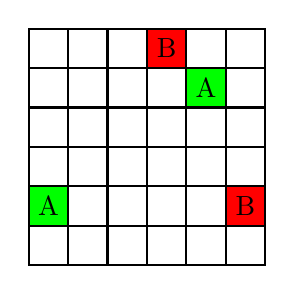
\begin{tikzpicture}
        [
            box/.style={rectangle,draw=black,thick, minimum size=0.5cm},
        ]
    
    \foreach \x in {0,0.5,...,2.5}{
        \foreach \y in {0,0.5,...,2.5}
            \node[box] at (\x,\y){};
    }
    \node [box,fill=green] at (0,0.5){A};
    \node[box,fill=green  ] at (2,2){A};  
    \node[box,fill=red  ] at (1.5,2.5){B}; 
    \node [box,fill=red] at (2.5,0.5){B}; 
    \end{tikzpicture}
}
\subfigure[Iteration number x] {
    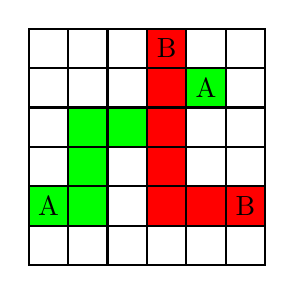
\begin{tikzpicture}
        [
            box/.style={rectangle,draw=black,thick, minimum size=0.5cm},
        ]
    
    \foreach \x in {0,0.5,...,2.5}{
        \foreach \y in {0,0.5,...,2.5}
            \node[box] at (\x,\y){};
    }
    
    \node [box,fill=green] at (0,0.5){A};
    \node[box,fill=green  ] at (2,2){A};  
    \node[box,fill=green  ] at (0.5,0.5){};  
    \node[box,fill=green  ] at (0.5,1){};  
    \node[box,fill=green  ] at (0.5,1.5){};  
    \node[box,fill=green  ] at (1,1.5){};  
    \node[box,fill=red  ] at (1.5,2.5){B}; 
    \node [box,fill=red] at (2.5,0.5){B};
    \node [box,fill=red] at (2,0.5){};
    \node [box,fill=red] at (1.5,0.5){};
    \node [box,fill=red] at (1.5,1){};
    \node [box,fill=red] at (1.5,1.5){};
    \node [box,fill=red] at (1.5,2){};
    \end{tikzpicture}
}
\subfigure[Iteration number y] {
    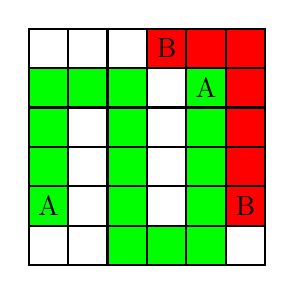
\begin{tikzpicture}
        [
            box/.style={rectangle,draw=black,thick, minimum size=0.5cm},
        ]
    
    \foreach \x in {0,0.5,...,2.5}{
        \foreach \y in {0,0.5,...,2.5}
            \node[box] at (\x,\y){};
    }
    
    \node [box,fill=green] at (0,0.5){A};
    \node[box,fill=green  ] at (2,2){A};  
    \node[box,fill=green  ] at (0,1){};  
    \node[box,fill=green  ] at (0,1.5){};  
    \node[box,fill=green  ] at (0,2){};  
    \node[box,fill=green  ] at (0.5,2){};  
    \node[box,fill=green  ] at (1,2){};  
    \node[box,fill=green  ] at (1,1.5){};  
    \node[box,fill=green  ] at (1,1){};  
    \node[box,fill=green  ] at (1,0.5){};  
    \node[box,fill=green  ] at (1.5,0){};  
    \node[box,fill=green  ] at (1,0){};  
    \node[box,fill=green  ] at (2,0){};  
    \node[box,fill=green  ] at (2,0.5){};  
    \node[box,fill=green  ] at (2,1){};  
    \node[box,fill=green  ] at (2,1.5){};  
    \node[box,fill=red  ] at (1.5,2.5){B}; 
    \node [box,fill=red] at (2.5,0.5){B};  
    \node [box,fill=red] at (2.5,1){};
    \node [box,fill=red] at (2.5,1.5){};
    \node [box,fill=red] at (2.5,2){};
    \node [box,fill=red] at (2.5,2.5){};
    \node [box,fill=red] at (2,2.5){};
    \end{tikzpicture}
}
\subfigure[After N iteration] {
    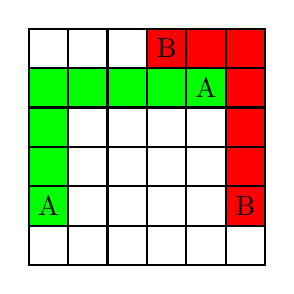
\begin{tikzpicture}
        [
            box/.style={rectangle,draw=black,thick, minimum size=0.5cm},
        ]
    
    \foreach \x in {0,0.5,...,2.5}{
        \foreach \y in {0,0.5,...,2.5}
            \node[box] at (\x,\y){};
    }
    
    \node [box,fill=green] at (0,0.5){A};
    \node[box,fill=green  ] at (2,2){A};  
    \node[box,fill=green  ] at (0,1){};  
    \node[box,fill=green  ] at (0,1.5){};  
    \node[box,fill=green  ] at (0,2){};  
    \node[box,fill=green  ] at (0.5,2){};  
    \node[box,fill=green  ] at (1,2){};  
    \node[box,fill=green  ] at (1.5,2){};  
    \node[box,fill=red  ] at (1.5,2.5){B}; 
    \node [box,fill=red] at (2.5,0.5){B}; 
    \node [box,fill=red] at (2.5,1){};
    \node [box,fill=red] at (2.5,1.5){};
    \node [box,fill=red] at (2.5,2){};
    \node [box,fill=red] at (2.5,2.5){};
    \node [box,fill=red] at (2,2.5){};
    \end{tikzpicture}
}
\caption{Finding path in global routing}
\label{fig:GlobalRoutingProcess}
\end{figure}
\medskip
Figure~\ref{fig:GlobalRoutingProcess} shows a very simple approach of how the global router works. At (a) the source and target of both (A,B) need to be connected ignoring obstacles, nevertheless we can observe that the global router have to iterate to get the best routing paths, at (b) (B,B) connected but there is no way to connect (A,A) as when (B,B) connected together they blocked the way for (A,A) to be connected, after some iterations we can find the figure at (c) in which (A,A) and (B,B) connected correctly, but there is a problem, the (A,A) connection is not the optimal path as there are paths which achieve less wire length, so the global router have to iterate until reaching the optimal path. These iterations are done for only two connections in one layer without obstacles, then how about millions of wires in VLSI? this shows how much the global routing algorithm has to be very fast in order to connect this huge number of wires as fast as possible.


%%%%%%%%%%%%%%%%%%%%%%%%%%%%%%%%%%%%%%%%%%%%%%%%%%%%%%%%%%%%%%%%%%%%%%%%%%%%%%%%%%%
%%%%%%%%%%%%%%%%%%%%%%%%%%%%%%%%%% RELATED WORK %%%%%%%%%%%%%%%%%%%%%%%%%%%%%%%%%%%
%%%%%%%%%%%%%%%%%%%%%%%%%%%%%%%%%%%%%%%%%%%%%%%%%%%%%%%%%%%%%%%%%%%%%%%%%%%%%%%%%%%

\section{Related Work}

Several papers proposed various types of approaches to improve the routing process, each of them tried to improve the overall routing by improving one or more parameters, some papers tried to decrease the number of vias, other papers tried to decrease the time taken and so on.
\medskip
\par
In \cite{b1}, a sequential global routing is used and two bounded length maze algorithms as finding path algorithms are provided in order to make the router faster and to avoid congestions thus avoiding overflow, the first one is optimal-BLMR and the second one is heuristic-BLMR. optimal-BLMR is used to get the minimum cost paths to be used as routing paths, this can be done in three steps. First BLC (bounded length constraint) is defined as a greater number than Manhattan distance then to go from source to target the neighbor points are tested if it can be a part of a path or not, each point that violates the BLC constraint is discarded. Second, if the route Started from point \textit{v}, ended at point \textit{u} and there were many paths between these two points, the normal maze algorithm will take the path with the minimum cost which may cause the route to pass through congestions, but in optimal-BLMR, it keeps track of all paths between these two points in order to choose the path that will not cause overflow, it iterates on the minimum cost path every time and if it found a suitable path it reserves that path, otherwise, it discards that path. Third step the optimal-BLMR iterates on the reserved paths and choose the one to be used for routing. Heuristic-BLMR is used to speed the router up by reserving only one path between the two points, but it has to keep the advantage of optimal-BLMR (avoiding congestions), this can be achieved by reserving the selected path only if the wire length is enough to detour around congested regions. The advantages of this paper are using sequential global routing which is based on multithreaded global routing which speedup the router between $2.71$ and $3.12$ in overflow free cases, avoiding collision by using optimal-BLMR, and making a fast and nearly avoiding collision algorithm (heuristic-BLMR). But there are some disadvantages too, as optimal-BLMR is very slow to be used, although heuristic-BLMR is faster than optimal-BLMR its results are not accurate as the wire length is not the best compared with other papers, and it is done on \textit{2D} grid then it is projected to the \textit{3D} one however, this approach gives a good result but it is not accurate like routers that apply routing in the \textit{3D} grid directly as in \cite{b9}.
\medskip
\par
In \cite{b4}, both of via count and runtime are reduced, this done by integrating \cite{b2}, \cite{b11}, and \cite{b12} with via aware Steiner tree generation, 3-bend routing, and layer assignment with careful edge and net ordering to create \cite{b4}. Via aware Steiner tree is used to at the beginning of the global routing, it generates a suitable topology, by changing tree topology the via count greatly changed, which means that using a suitable topology for Steiner tree will greatly reduce the via count. The 3-bend routing is used instead of L, U, Z, maze, and monotonic routing, as L, U, Z routing can not avoid congestions but they generate a little number of vias, maze and monotonic can avoid congestions but they generate a lot of vias and their runtime is very high, so the 3-bend routing was used as it is fast, its completely \textit{O(nm)}, and it generates vias less than maze and monotonic routing as it consists of two L routing. Layer assignment with careful ordering algorithm is used as a solution of \textit{3D}, it is like all the modern techniques project the \textit{3D} grid into \textit{2D} one to be easier and faster in routing, this algorithm guarantees the wire length and overflow unchanged on assigning to layers, dynamic programming is used in layer assignment to make it faster. From the previous explanation, the advantages of this paper are decreasing the number of vias, which means less power consumption and circuit delay, and decreasing runtime of global routing thus decreasing runtime of whole the routing process. But it has disadvantages too, one of them is the wire length is not optimal, as using 3-bend routing increases the wire length to avoid congestions, another one is caused by layer assignment as if the \textit{2D} was not congestion-free the results will not be accurate.

\medskip
\par
In \cite{b13} they proposed an approach to not only perform pathfinding, but also the global routers are also required to generate a set of connected rectangle guides,  each of which contains an integral number of G-cells so that the detailed router can find a path within the guides to connect all pins of each net and reduce a given cost function to the minimum. \\
The proposed 3D pattern routing generates 3D topologies directly, while the traditional 3D pattern routing only generates 2D topologies and uses an extra layer for the assignment level. They, therefore, proposed a combination of 2D pattern routing with layer assignment and used it to choose a path for each two-pin net, and, with the help of dynamic programming, they ensure that an optimal solution can be found if it exists.
The overall flow of their proposed algorithm can be divided into 3 parts, summarized as follows:
\begin{enumerate}
	\item Initial routing:
    \begin{enumerate}
    	\item Pattern Routing Planning: \\
        In order to carry out 3D pattern routing, each multi-pin net first will be broken into set of two pin nets in this step.        
        \item 3D Pattern Routing with Layer Assignment: \\
        After breaking down the nets into two-pin nets and decide their order,
        pattern routing and layer assignment are performed simultaneously using a dynamic programming algorithm.
        Rather than performing layer assignment after a net is a pattern routed,
        our dynamic programming algorithm merges the two steps to minimize the overall cost
        and Prevent loss of precision caused by compressing the 3D grid graph to 2D.
    \end{enumerate}
    \item Multi-level 3D Maze Routing: \\
    After initial routing, the nets with violations will be destroyed and multiple iterations of rip-up and reroute (RRR) may be performed by maze routing. The multi-level 3D Maze Routing is repeated until there's no overflow. Because the maze routing on the entire 3d  graph would take too much time because of the wide search space, an algorithm that limits the search area to the bounding box of the net will make rerouting much faster, but it may reduce the routing quality.
    Considering the above, the proposed algorithm Uses multi-level 3d maze routing to allow graph searching process while reaching reasonable trade off between time and routing quality.
    The proposed routing technique has two levels, each serves a different purpose:
    \begin{enumerate}
    	\item  Maze Routing Planning (Bounding Box Generation): \\
        In order to carry out 3D pattern routing, each multi-pin net will first be broken down into a set of two-pin nets in this step.        
        \item 3D Maze Routing within Bounding Box (fine-grained maze routing within guides): \\
        Performs another level of maze routing, it seeks to find a path with the minimum
        actual cost within the search space.
    \end{enumerate}
	\item Route guide generation \& patching: \\
    The output of the global router is connected rectangular route guides, the algorithm proposes a new technique called patching to add some stand-alone route guides or patches onto the routed path to further improve the detailed routing.
\end{enumerate}

They introduce a global 3D router that could enhance the routing well in efficiency and quality. The 3d routing technique combines 2d routing and assignment of layers and helps most nets to be routed quickly and optimally. A patching method that actually contributes to useful route guidance to improve detailed routing in some way. An innovative probability-based cost scheme which takes into account the risk of overflow, the total wire length, and it is also capable of reducing the number of via and the total wire length while avoiding overflow and preserving enough edge capacity which is the number of paths that can pass through the edge. A multi-level maze routing method which is used to shrink the search space and then performs a bounded maze routing to find a minimum cost path.in that method we decided to work on the time parameter by instead of using the Dijkstra algorithm we will use the A-Star algorithm with a proposed heuristic function that will improve the time.

%%%%%%%%%%%%%%%%%%%%%%%%%%%%%%%%%%%%%%%%%%%%%%%%%%%%%%%%%%%%%%%%%%%%%%%%%%%%%%%%%%%
%%%%%%%%%%%%%%%%%%%%%%%%%%%%%%%% PROPOSED APPROACH %%%%%%%%%%%%%%%%%%%%%%%%%%%%%%%%
%%%%%%%%%%%%%%%%%%%%%%%%%%%%%%%%%%%%%%%%%%%%%%%%%%%%%%%%%%%%%%%%%%%%%%%%%%%%%%%%%%%


\section{Proposed Approach}
For global routing, three parameters are considered. The first is the total wire length, the second is the total overflow. The third is the running time. In our proposed solution, we are focused on the time parameter without affecting much the total wire length and total overflow. So according to minimize the time we have decided to apply A-Star algorithm as the pathfinder algorithm with a proposed heuristic function, A-Star is basically a guided variation of Dijkstra. This algorithm can be turned into a better or worse pathfinding algorithm by experimenting with the heuristics it uses and how it evaluates each node A-Star expands on a node only if it seems promising. Its only focus is to reach the goal node as quickly as possible from the current node, not to try and reach every other node. Illustrative example:
\begin{figure} [hbt!]
    \centering  
    \subfigure[Maze] {
    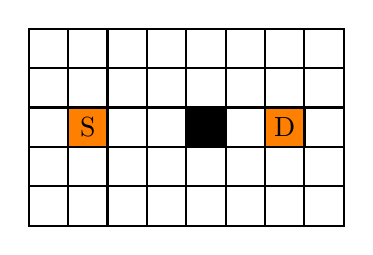
\begin{tikzpicture}
        [
            box/.style={rectangle,draw=black,thick, minimum size=0.5cm},
        ]
    
    \foreach \x in {0,0.5,...,3.5}{
        \foreach \y in {0,0.5,...,2}
            \node[box] at (\x,\y){};
    }
    \node [box,fill=orange] at (0.5,1){S};
    \node[box,fill=orange  ] at (3,1){D};  
    \node[box,fill=black  ] at (2,1){ };  
    \end{tikzpicture}
}

\subfigure[Applying Dijkstra] {
    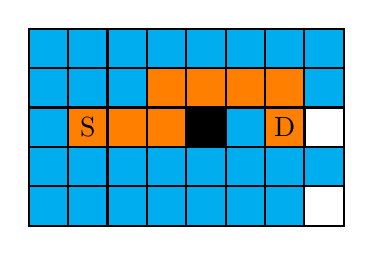
\begin{tikzpicture}
        [
            box/.style={rectangle,draw=black,thick, minimum size=0.5cm},
        ]
    
    \foreach \x in {0,0.5,...,3.5}{
        \foreach \y in {0,0.5,...,2}
            \node[box] at (\x,\y){};
    }

    \node [box,fill=cyan] at (0,0){};
    \node [box,fill=cyan] at (0.5,0){};
    \node [box,fill=cyan] at (1,0){};
    \node [box,fill=cyan] at (1.5,0){};
    \node [box,fill=cyan] at (2,0){};
    \node [box,fill=cyan] at (2.5,0){};
    \node [box,fill=cyan] at (3,0){};
    \node [box,fill=cyan] at (0,0.5){};
    \node [box,fill=cyan] at (0.5,0.5){};
    \node [box,fill=cyan] at (1,0.5){};
    \node [box,fill=cyan] at (1.5,0.5){};
    \node [box,fill=cyan] at (2,0.5){};
    \node [box,fill=cyan] at (2.5,0.5){};
    \node [box,fill=cyan] at (3,0.5){};
    \node [box,fill=cyan] at (3.5,.5){};
    \node [box,fill=cyan] at (2.5,1){};
    \node [box,fill=cyan] at (0,1){};
    \node [box,fill=cyan] at (2.5,0.5){};
    \node [box,fill=cyan] at (0,2){};
    \node [box,fill=cyan] at (0.5,2){};
    \node [box,fill=cyan] at (1,2){};
    \node [box,fill=cyan] at (1.5,2){};
    \node [box,fill=cyan] at (2,2){};
    \node [box,fill=cyan] at (2.5,2){};
    \node [box,fill=cyan] at (3,2){};
    \node [box,fill=cyan] at (3.5,2){};
    \node [box,fill=cyan] at (3.5,1.5){};
    \node [box,fill=cyan] at (0,1.5){};
    \node [box,fill=cyan] at (0.5,1.5){};
    \node [box,fill=cyan] at (1,1.5){};
    \node [box,fill=orange] at (0.5,1){S};
    \node [box,fill=orange] at (1,1){};
    \node [box,fill=orange] at (1.5,1){};
    \node [box,fill=orange] at (1.5,1.5){};
    \node [box,fill=orange] at (2,1.5){};
    \node [box,fill=orange] at (2.5,1.5){};
    \node [box,fill=orange] at (3,1.5){};
    \node[box,fill=orange  ] at (3,1){D};  
    \node[box,fill=black  ] at (2,1){ };  
    \end{tikzpicture}
}
\subfigure[Applying A-Star] {
    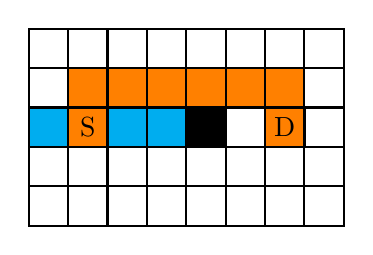
\begin{tikzpicture}
        [
            box/.style={rectangle,draw=black,thick, minimum size=0.5cm},
        ]
    
    \foreach \x in {0,0.5,...,3.5}{
        \foreach \y in {0,0.5,...,2}
            \node[box] at (\x,\y){};
    }
    \node [box,fill=orange] at (0.5,1){S};
    \node[box,fill=orange  ] at (3,1){D};
    \node [box,fill=orange] at (0.5,1.5){};  
    \node [box,fill=orange] at (1,1.5){};  
    \node [box,fill=orange] at (1.5,1.5){};
    \node [box,fill=orange] at (2,1.5){};
    \node [box,fill=orange] at (2.5,1.5){};
    \node [box,fill=orange] at (3,1.5){};
    \node [box,fill=cyan] at (0,1){};
    \node [box,fill=cyan] at (1,1){};
    \node [box,fill=cyan] at (1.5,1){};
    \node[box,fill=black  ] at (2,1){ };  
    \end{tikzpicture}
}
\caption{Comparison between Dijkstra \& A-Star }
\label{fig:GlobalRoutingProcess}
\end{figure}
\medskip
In the illustrative example the visited nodes are marked in cyan color, the path is in orange color, and the blocked cells are black.
Both have path of six cells which in our case they have optimal wire length but totally different running time as Dijkstra visits much more nodes than A-Star
, in the case of many target nodes, Dijkstra might be better in total wire length but much slower than A-Star, with an appropriate heuristic function we can minimize the time and try to reach optimal wire length. The heuristic function is a way of informing the search about the path to a target that provides an intelligent way of guessing which neighbor of the node is going to lead to the target faster. Hence, our heuristic function composed of Manhattan distance, layer index, and some constants.
\begin{multline*}
    h = \ln (\mid p1 \cdot x-p2 \cdot x\mid+\mid p1 \cdot y-p2 \cdot y\mid)*const1 \\ 
     +(\mid p1 \cdot layerid-p2 \cdot layerid\mid)*const2 \\
\end{multline*}
The global router is implemented using C++ with the boost library, and a parser for LEF/DEF formats. We conducted our experiment with the same configuration and tried to test the global router behavior using A-Star algorithm instead of Dijkstra's.


%%%%%%%%%%%%%%%%%%%%%%%%%%%%%%%%%%%%%%%%%%%%%%%%%%%%%%%%%%%%%%%%%%%%%%%%%%%%%%%%%%%
%%%%%%%%%%%%%%%%%%%%%%%%%%%%%%%%%%%% ALGORITHM %%%%%%%%%%%%%%%%%%%%%%%%%%%%%%%%%%%%
%%%%%%%%%%%%%%%%%%%%%%%%%%%%%%%%%%%%%%%%%%%%%%%%%%%%%%%%%%%%%%%%%%%%%%%%%%%%%%%%%%%

\subsection{Proposed Algorithm}
% \floatstyle{norules}
\restylefloat{algorithm}
\begin{algorithm}[H]
    \caption{A-Star Algorithm}
    \hspace*{\algorithmicindent} \textbf{Input:} Grid values $g$, Source $s$, Destination $d$\\
    \hspace*{\algorithmicindent} \textbf{Output:} Path\\
    \begin{algorithmic}[1]
    \Procedure {A-Star}{}
    % Return  Average waiting time, throughput
    \Statex Declaration and Initialisation:
    \State Cells $\theta$ % The Cells in the grid.
    \State Visited Nodes $\phi$ % Nodes already visited.
    \State Openlist Nodes $\delta$ % Nodes still to be visited. pq
    \State The cost from Starting point to a given node $g$
    \State The heuristic function $h$
    \State (The cost of $g$ + The cost of $h$) is $f$
    \If{$s$ or $d$ is invalid}
        \Return
    \EndIf
    \If{$s$ or $d$ is blocked}
        \State \Return
    \EndIf
    \If{$s$ = $d$}
        \State \Return
    \EndIf
    \State Initialize $\delta$ 
    \State Initialize $\phi$
        \While{$\delta$ is not empty}
            \State $currNode$  = node with least $f$ in $\delta$
            \State $\delta$.Remove($currNode$)
            \State Generate 4 neighbours of $currNode$
            \For{$neighbour \in neighbours$}
            \If{$neighbour$ = $d$}
                \State Get path
                \State \Return
            \ElsIf{$neighbour \notin \phi$ and $neighbour$ is not blocked}
                \State $gnew$ = $currNode$.$g$ + distance between neighbour and currNode
                \State $hnew$ = distance from $d$ to $neighbour$
                \State $fnew$ = $gnew$ + $hnew$
                \If{$fnew < neighbour$.$f$}
                \State $neighbour$.$g$ = $currNode$.$g$ + distance between neighbour and currNode
                \State $neighbour$.$h$ = distance from $d$ to $neighbour$
                \State $neighbour$.$f$ = $neighbour$.$g$ + $neighbour$.$h$
                \State $\delta$.Add($neighbour$)
                \EndIf
            \EndIf
            \EndFor
        \State $\phi$.Add($currNode$)
        \EndWhile
        \EndProcedure
    \end{algorithmic}
\end{algorithm}

%%%%%%%%%%%%%%%%%%%%%%%%%%%%%%%%%%%%%%%%%%%%%%%%%%%%%%%%%%%%%%%%%%%%%%%%%%%%%%%%%%%
%%%%%%%%%%%%%%%%%%%%%%%%%%%%%% EXPERIMENTAL ANALYSIS %%%%%%%%%%%%%%%%%%%%%%%%%%%%%%
%%%%%%%%%%%%%%%%%%%%%%%%%%%%%%%%%%%%%%%%%%%%%%%%%%%%%%%%%%%%%%%%%%%%%%%%%%%%%%%%%%%


\section{Experimental Analysis}

we implement global routing with A-Star router algorithm in c++ language
with Rsyn to parse input test cases files with format LEF/DEF. All
experiments are performed on a Machine with 2 GHZ Intel Processor
and 8 GB RAM. our algorithm is focus on three important factors :total
wire-length, channel congestion ,number of vias. Our target is to
minimize a convex combination of the total wire-length and the number
of vias that represent the bends in the tree that result in solving
the net of pins to be connected.our test cases input are all from
ICCAD'19 contest for global routing.we test our code with different
heuristic functions -that affect the run time of A-Star- to check its
effect on CPU run time.our concern is on wire-length and number of
vias result from routing without increasing in-feasibility.we generate
the trees of all nets in parallel to reduce running by using multi-threaded
approach to generate the net results tree as this step has the most
costly part of the router algorithm.our algorithm not only route each net to find a path that connect all pins of the net, but it also generate a set of connected rectangle for each net to be used in detailed routing and to minimize its cost. 

\subsubsection{Experiment 1}

In this experiment we compare run time of router with Dijkstra Router
and out A-Star router with heuristic function with different constants
of heuristic functions that affect the run time of the router.heuristic
function help us to know how near the point to the target point so it help in decreasing the cost of routing:

\begin{multline*}
h1=(\mid p1\cdot x-p2\cdot x\mid+\mid p1\cdot y-p2\cdot y\mid)*const1\\
+(\mid p1\cdot layerid-p2\cdot layerid\mid)*const2\\
\end{multline*}

\begin{multline*}
h2=ln(\mid p1\cdot x-p2\cdot x\mid+\mid p1\cdot y-p2\cdot y\mid)*const1\\
+(\mid p1\cdot layerid-p2\cdot layerid\mid)*const2\\
\end{multline*}

\begin{multline*}
h3=(\mid p1\cdot x-p2\cdot x\mid+\mid p1\cdot y-p2\cdot y\mid)*const1\\
+ln(\mid p1\cdot layerid-p2\cdot layerid\mid)*const2\\
\end{multline*}


{\tiny{}}
\begin{table}[b]
{\tiny{}\caption{\label{tab:Compare-run-time}Compare run time of Dijkstra router and
A-Star router with Heuristic-Function 1}
}{\tiny\par}
\centering{}{\footnotesize{}}%
\begin{adjustbox}{width=\columnwidth,center}
\begin{tabular}{|c|c|c|c|c|c|}
\hline 
\multirow{2}{*}{{\footnotesize{}Design}} & \multicolumn{4}{c|}{{\footnotesize{}A-Star}} & \multirow{2}{*}{{\footnotesize{}Dijkstra}}\tabularnewline
\cline{2-5} \cline{3-5} \cline{4-5} \cline{5-5} 
 & {\footnotesize{}(0.2,0.1)} & {\footnotesize{}(0.3,0.3)} & {\footnotesize{}(0.5,0.5)} & \multicolumn{1}{c||}{{\footnotesize{}(0.5,0.5)}} & \tabularnewline
\hline 
\hline 
{\footnotesize{}test1} & {\footnotesize{}75.843764} & {\footnotesize{}87.797614} & {\footnotesize{}87.086193} & {\footnotesize{}96.377979} & {\footnotesize{}91.348007}\tabularnewline
\hline 
{\footnotesize{}test2} & {\footnotesize{}2.511599} & {\footnotesize{}2.606054} & {\footnotesize{}2.874605} & {\footnotesize{}2.497377} & {\footnotesize{}3.435606}\tabularnewline
\hline 
{\footnotesize{}test3} & {\footnotesize{}12.381436} & {\footnotesize{}14.959666} & {\footnotesize{}14.859677} & {\footnotesize{}14.766495} & {\footnotesize{}11.824573}\tabularnewline
\hline 
{\footnotesize{}test4} & {\footnotesize{}0.075472} & {\footnotesize{}0.073069} & {\footnotesize{}0.073769} & {\footnotesize{}0.072691} & {\footnotesize{}0.071829}\tabularnewline
\hline 
{\footnotesize{}test5} & {\footnotesize{}0.073988} & {\footnotesize{}0.072911} & {\footnotesize{}0.074165} & {\footnotesize{}0.072767} & {\footnotesize{}0.071945}\tabularnewline
\hline 
{\footnotesize{}test6} & {\footnotesize{}6.948016} & {\footnotesize{}6.266789} & {\footnotesize{}5.198969} & {\footnotesize{}6.906992} & {\footnotesize{}7.0385}\tabularnewline
\hline 
\end{tabular}{\footnotesize\par}
\end{adjustbox}
\end{table}
{\tiny\par}

\begin{table}
\caption{\label{tab:Compare-run-time-1}Compare run time of Dijkstra router
and A-Star router with Heuristic-Function 2}

\centering{}{\footnotesize{}}%
\begin{adjustbox}{width=\columnwidth,center}
\begin{tabular}{|c|c|c|c|c|c|}
\hline 
\multirow{2}{*}{{\footnotesize{}Design}} & \multicolumn{4}{c|}{{\footnotesize{}A-Star}} & \multirow{2}{*}{{\footnotesize{}Dijkstra}}\tabularnewline
\cline{2-5} \cline{3-5} \cline{4-5} \cline{5-5} 
 & {\footnotesize{}(0.1,0.1)} & {\footnotesize{}(0.2,0.1)} & {\footnotesize{}(0.3,0.3)} & {\footnotesize{}(0.5,0.5)} & \tabularnewline
\hline 
\hline 
{\footnotesize{}test1} & {\footnotesize{}90.440165} & {\footnotesize{}93.288501} & {\footnotesize{}89.414646} & {\footnotesize{}96.377979} & {\footnotesize{}91.348007}\tabularnewline
\hline 
{\footnotesize{}test2} & {\footnotesize{}2.461400} & {\footnotesize{}2.469304} & {\footnotesize{}2.480592} & {\footnotesize{}2.497377} & {\footnotesize{}3.435606}\tabularnewline
\hline 
{\footnotesize{}test3} & {\footnotesize{}12.264829} & {\footnotesize{}13.449206} & {\footnotesize{}12.039944} & {\footnotesize{}14.766495} & {\footnotesize{}11.824573}\tabularnewline
\hline 
{\footnotesize{}test4} & {\footnotesize{}0.071577} & {\footnotesize{}0.157244} & {\footnotesize{}0.078624} & {\footnotesize{}0.072691} & {\footnotesize{}0.071829}\tabularnewline
\hline 
{\footnotesize{}test5} & {\footnotesize{}0.078316} & {\footnotesize{}0.090906} & {\footnotesize{}0.071333} & {\footnotesize{}0.072767} & {\footnotesize{}0.071945}\tabularnewline
\hline 
{\footnotesize{}test6} & {\footnotesize{}6.893310} & {\footnotesize{}6.400888} & {\footnotesize{}6.974920} & {\footnotesize{}6.906992} & {\footnotesize{}7.038505}\tabularnewline
\hline 
\end{tabular}{\footnotesize\par}
\end{adjustbox}
\end{table}

\begin{table}
{\tiny{}\caption{\label{tab:Continue-compare-run} compare run time of Dijkstra router
and A-Star router with Heuristic-Function 3}
}{\tiny\par}
\centering{}{\footnotesize{}}%
\begin{adjustbox}{width=\columnwidth,center}
\begin{tabular}{|c|c|c|c|c|c|}
\hline 
\multirow{2}{*}{{\footnotesize{}Design}} & \multicolumn{4}{c|}{{\footnotesize{}A-Star}} & \multirow{2}{*}{{\footnotesize{}Dijkstra}}\tabularnewline
\cline{2-5} \cline{3-5} \cline{4-5} \cline{5-5} 
 & {\footnotesize{}(0.1,0.1)} & {\footnotesize{}(0.2,0.1)} & {\footnotesize{}(0.3,0.3)} & {\footnotesize{}(0.5,0.5)} & \tabularnewline
\hline 
\hline 
{\footnotesize{}test1} & {\footnotesize{}86.598509} & {\footnotesize{}83.204272} & {\footnotesize{}103.166426} & {\footnotesize{}102.378304} & {\footnotesize{}91.348007}\tabularnewline
\hline 
{\footnotesize{}test2} & {\footnotesize{}2.481847} & {\footnotesize{}2.486656} & {\footnotesize{}3.622759} & {\footnotesize{}2.556863} & {\footnotesize{}3.435606}\tabularnewline
\hline 
{\footnotesize{}test3} & {\footnotesize{}12.655603} & {\footnotesize{}15.447421} & {\footnotesize{}15.629251} & {\footnotesize{}20.004493} & {\footnotesize{}11.824573}\tabularnewline
\hline 
{\footnotesize{}test4} & {\footnotesize{}0.073731} & {\footnotesize{}0.070911} & {\footnotesize{}0.073468} & {\footnotesize{}0.103421} & {\footnotesize{}0.071829}\tabularnewline
\hline 
{\footnotesize{}test5} & {\footnotesize{}0.078171} & {\footnotesize{}0.079362} & {\footnotesize{}0.088107} & {\footnotesize{}0.099699} & {\footnotesize{}0.071945}\tabularnewline
\hline 
{\footnotesize{}test6} & {\footnotesize{}6.470339} & {\footnotesize{}7.195767} & {\footnotesize{}8.455288} & {\footnotesize{}7.637577} & {\footnotesize{}7.038505}\tabularnewline
\hline 
\end{tabular}{\footnotesize\par}
\end{adjustbox}
\end{table}

we notice from Table\ref{tab:Compare-run-time},Table\ref{tab:Continue-compare-run},Table\ref{tab:Compare-run-time-1}
that heuristic function affect the running time of router ,decreases
it to be lower than Dijkstra router's running time in many test cases.
the running time changes with the change of heuristic function constants.
we notice that higher constants increase the running time and sometimes
be greater than Dijkstra router's run time. Heuristic function 2 has
overall results which is better than others, with using more efficient
heuristic functions,run time and wire-length and vias number combination
may improve greatly. 

\subsection{Performance Comparisons}

we used ISPD19 benchmarks to compare out results with another global
routing algorithms such as TripleZ and NTUidRoute. we compare the
results in terms of total wire length score and vias score. we compare
results of our algorithm which focus on factors - total wire-length,number
of vias in the routing results - with TripleZ and NTUidRoute algorithms
in ICCAD'19 Table\ref{tab:compared-Wire-Lengh},Table \ref{tab:compared-Vias}
.we use multi-threaded approach to generate net result trees in parallel
so we have done our experiments using 8 threads in all test cases.
score used as unit to compare ,score of wire length is a function
of metal pitch and wire length and weight:

\[
WLScore=\frac{wire-length*weight}{metal-pitch}
\]

score of vias is function of number of vias :

\[
ViasScore=\#vias*2
\]

{\tiny{}}
\begin{table}
{\tiny{}\caption{\label{tab:compared-Wire-Lengh}compared Wire Length with TripleZ and
NTUidRoute Algorithms in ICCAD'19 Global routing Contest }
}{\tiny\par}
\centering{}{\footnotesize{}}%
\begin{tabular}{|c|c|c|c|}
\hline 
\multirow{2}{*}{{\footnotesize{}Design}} & \multicolumn{3}{c|}{{\footnotesize{}wire-length scores}}\tabularnewline
\cline{2-4} \cline{3-4} \cline{4-4} 
 & {\footnotesize{}TripleZ} & {\footnotesize{}NTUidRoute} & {\footnotesize{}ours}\tabularnewline
\hline 
{\footnotesize{}test1} & {\footnotesize{}12485549.76} & {\footnotesize{}12992510.61} & {\footnotesize{}12150100}\tabularnewline
\hline 
{\footnotesize{}test2} & {\footnotesize{}569622.01} & {\footnotesize{}466809.64} & {\footnotesize{}389460}\tabularnewline
\hline 
{\footnotesize{}test7} & {\footnotesize{}17800019.36} & {\footnotesize{}15935101.91} & {\footnotesize{}14663400}\tabularnewline
\hline 
{\footnotesize{}test3} & {\footnotesize{}2859212.04} & {\footnotesize{}2495661.79} & {\footnotesize{}2851900}\tabularnewline
\hline 
{\footnotesize{}test8} & {\footnotesize{}74264784.88} & {\footnotesize{}65028116.52} & {\footnotesize{}70041500}\tabularnewline
\hline 
{\footnotesize{}Avg} & {\footnotesize{}21595837.61} & {\footnotesize{}19383640} & {\footnotesize{}20019272}\tabularnewline
\hline 
\end{tabular}{\footnotesize\par}
\end{table}
{\tiny\par}

\begin{table} [hbt!]
\centering{}{\footnotesize{}\caption{\label{tab:compared-Vias}compared Vias TripleZ and NTUidRoute Algorithms
in ICCAD'19 Global routing Contest}
}%
\begin{tabular}{|c|c|c|c|}
\hline 
\multirow{2}{*}{{\footnotesize{}Design}} & \multicolumn{3}{c|}{{\footnotesize{}vias score}}\tabularnewline
\cline{2-4} \cline{3-4} \cline{4-4} 
 & {\footnotesize{}TripleZ} & {\footnotesize{}NTUidRoute} & {\footnotesize{}ours}\tabularnewline
\hline 
\hline 
{\footnotesize{}test1} & {\footnotesize{}3261476.00} & {\footnotesize{}4017448.00} & {\footnotesize{}2803560}\tabularnewline
\hline 
{\footnotesize{}test2} & {\footnotesize{}251728.00} & {\footnotesize{}318404.00} & {\footnotesize{}176728}\tabularnewline
\hline 
{\footnotesize{}test7} & {\footnotesize{}4265744.00} & {\footnotesize{}4789488.00} & {\footnotesize{}2666120}\tabularnewline
\hline 
{\footnotesize{}test3} & {\footnotesize{}695348.00} & {\footnotesize{}771328.00} & {\footnotesize{}446024}\tabularnewline
\hline 
{\footnotesize{}test8} & {\footnotesize{}19689760.00} & {\footnotesize{}23183264.00} & {\footnotesize{}12532800}\tabularnewline
\hline 
{\footnotesize{}Avg} & {\footnotesize{}5632811.2} & {\footnotesize{}6615986.4} & {\footnotesize{}3725046.4}\tabularnewline
\hline 
\end{tabular}
\end{table}


\subsection{Observation}

for each benchmark we obtained wire length score and vias score for
specific metal pitch and weight that used in score equation.we notice
that our algorithm achieved wire-length score less than TripleZ with
7.3\% and greater than NTUidRoute with 3.28\% in average.our vias
score is less than TripleZ's score by 33.86\% so our total results
is better than TripleZ's results in the two factors.wire length of
our algorithm is greater than NTUidRoute due to that we attempted
to minimize the total score combination of wire length and vias number
so the total average score of our results is less than NTUidRoute's
results.Decreasing wire length affect the vias number greatly so
our vias score is less than NTUidRoute's vias score by 43\% due to that
we try to decrease it as the vias is one of the sources of heat generation
in the chip.

%%%%%%%%%%%%%%%%%%%%%%%%%%%%%%%%%%%%%%%%%%%%%%%%%%%%%%%%%%%%%%%%%%%%%%%%%%%%%%%%%%%
%%%%%%%%%%%%%%%%%%%%%%%%%%%%%%%%%%% CONCLUSION %%%%%%%%%%%%%%%%%%%%%%%%%%%%%%%%%%%%
%%%%%%%%%%%%%%%%%%%%%%%%%%%%%%%%%%%%%%%%%%%%%%%%%%%%%%%%%%%%%%%%%%%%%%%%%%%%%%%%%%%

\section{Conclusion and Future Work}

In the process of physical design, routing is among the most critical steps and is usually a very challenging problem. Effective and powerful routing algorithms are important to deal with the challenges emerging from the increasingly growing scale of IC integration, Routers will continue to evolve with rapidly growing design challenges like signal integrity, nanometer effects, reliability, etc. The goal of this paper is to develop A-Star-based global Router with minimum wire length and the number of vias as the more vias number the more heat generated from the chip with minimum run time. In order to optimize the time parameter, we use a heuristic function that decreases the run time of router and test it with different constants to define its effect on run time, for future work we aim to define an effective heuristic function to improve the running time. And build upon A-Star algorithm using more efficient versions of A-Star algorithm such as bi-directional A-Star, iterative deepening A-Star. In bi-directional A-Star that processes edges in both directions that improve the running time as well as it saves the memory demand for path saving as we will deal with both directions of edge.

%%%%%%%%%%%%%%%%%%%%%%%%%%%%%%%%%%%%%%%%%%%%%%%%%%%%%%%%%%%%%%%%%%%%%%%%%%%%%%%%%%%
%%%%%%%%%%%%%%%%%%%%%%%%%%%%%%%%%%%% REFERENCES %%%%%%%%%%%%%%%%%%%%%%%%%%%%%%%%%%%
%%%%%%%%%%%%%%%%%%%%%%%%%%%%%%%%%%%%%%%%%%%%%%%%%%%%%%%%%%%%%%%%%%%%%%%%%%%%%%%%%%%

\begin{thebibliography}{00}

    \bibitem{b1} Liu, Wen-Hao, et al. "NCTU-GR 2.0: Multithreaded collision-aware global routing with bounded-length maze routing." \textit{IEEE Transactions on computer-aided design of integrated circuits and systems} 32.5 (2013): 709-722.
    
    \bibitem{b2} Zhang, Yanheng, Yue Xu, and Chris Chu. "FastRoute3. 0: a fast and high quality global router based on virtual capacity." \textit{2008 IEEE/ACM International Conference on Computer-Aided Design.} IEEE, 2008.

    \bibitem{b3} H.-Y. Chen, C.-H. Hsu, and Y.-W. Chang, “High-performance global routing with fast overflow reduction,” \textit{in 2009 Asia and South Pacific Design Automation Conference}, pp. 582–587, IEEE, 2009.

    \bibitem{b4} Xu, Yue, Yanheng Zhang, and Chris Chu. "FastRoute 4.0: global router with efficient via minimization." \textit{2009 Asia and South Pacific Design Automation Conference. IEEE}, 2009.

    \bibitem{b5} Cho, Minsik, et al. "BoxRouter 2.0: Architecture and implementation of a hybrid and robust global router." \textit{2007 IEEE/ACM International Conference on Computer-Aided Design. IEEE}, 2007.

    \bibitem{b6} Ozdal, Muhammet Mustafa, and Martin DF Wong. "Archer: a history-driven global routing algorithm." \textit{2007 IEEE/ACM International Conference on Computer-Aided Design. IEEE}, 2007.

    \bibitem{b7} Gao, Jhih-Rong, Pei-Ci Wu, and Ting-Chi Wang. "A new global router for modern designs." \textit{2008 Asia and South Pacific Design Automation Conference.} IEEE, 2008.

    \bibitem{b8} Moffitt, Michael D. "MaizeRouter: Engineering an effective global router." \textit{IEEE Transactions on Computer-Aided Design of Integrated Circuits and Systems} 27.11 (2008): 2017-2026.

    \bibitem{b9} Roy, Jarrod A., and Igor L. Markov. "High-performance routing at the nanometer scale." \textit{IEEE Transactions on Computer-Aided Design of Integrated Circuits and Systems} 27.6 (2008): 1066-1077.

    \bibitem{b10} Chang, Yen-Jung, Yu-Ting Lee, and Ting-Chi Wang. "NTHU-Route 2.0: a fast and stable global router." \textit{2008 IEEE/ACM International Conference on Computer-Aided Design. IEEE}, 2008.

    \bibitem{b11} Pan, Min, and Chris Chu. "FastRoute: A step to integrate global routing into placement." \textit{Proceedings of the 2006 IEEE/ACM international conference on Computer-aided design.} 2006.

    \bibitem{b12} Pan, Min, and Chris Chu. "FastRoute 2.0: A high-quality and efficient global router." \textit{2007 Asia and south pacific design automation conference.} IEEE, 2007.

    \bibitem{b13} Liu, Jinwei, et al. "CUGR: Detailed-Routability-Driven 3D Global Routing with Probabilistic Resource Model."

    \bibitem{b14} Wu, Tai-Hsuan, Azadeh Davoodi, and Jeffrey T. Linderoth. "GRIP: scalable 3D global routing using integer programming." \textit{Proceedings of the 46th Annual Design Automation Conference}. 2009.

    \bibitem{b15} Xu, Yue, and Chris Chu. "MGR: Multi-level global router." \textit{2011 IEEE/ACM International Conference on Computer-Aided Design (ICCAD)}. IEEE, 2011.

\end{thebibliography}

\end{document}
